\chapter{Narukvica}
\label{pog:bracelet}
Svrha narukvice je prikupljanje biomedicinskih parmetara korisnika i njihovo slanje na obradu na glavnoj ploči. Biomedicinski parametri koji će se promatrati su brzina otkucaja srca putem fotopletizmografskog senzora (PPG) i impedancija kože, odnosno elektrodermalna aktivnost. Promjena elektrodermalna aktivnost je dobar pokazatelj stresa u korisnika \cite{edr}, a osobe sa poremećajem tečnosti govora pokazuju značajno smanjenje brzine otkucaja srca u stresnim situacijama u odnosu na osobe bez takvih poremećaja \cite{ALM2004123}.

Što se tiče zahtjeva na napajanje narukvice, situacija je ista kao i kod glavne ploče, uz drugačiju potrošnju. Tako da izrada pločice za narukvicu predstavlja mogućnost ispravljanja grešaka nastalih tijekom dizajna napajanja glavne ploče. Narukvica također mora imati mogućnost bežične komunikacije. S obzirom na ograničenje veličine ploče maknuti su kratkospojnici i testne točke.

\section{Bežična komunikacija}
Shema bežične komunikacije na narukvici (slika \ref{slk:BR_WIRELESS}) je veoma slična onoj na glavnoj ploči (slika \ref{slk:WIFI}), uz nedostatak kratkospojnika, dodatak signala za upravljanje I\textsubscript{2}C sučeljem i korištenje analogno-digitalnog pretvornika za mjerenje impadancije kože. Još jedna promjena dolazi u obliku programiranja preko UART-a. S obzirom na probleme tijekom programiranja glavne ploče dodani su signali DTR i CTS kako bi se BOOT i EN stezaljke ESP mikrokontrolera mogle programski upravljati.
\begin{sidewaysfigure}[htbp]
    \centering
    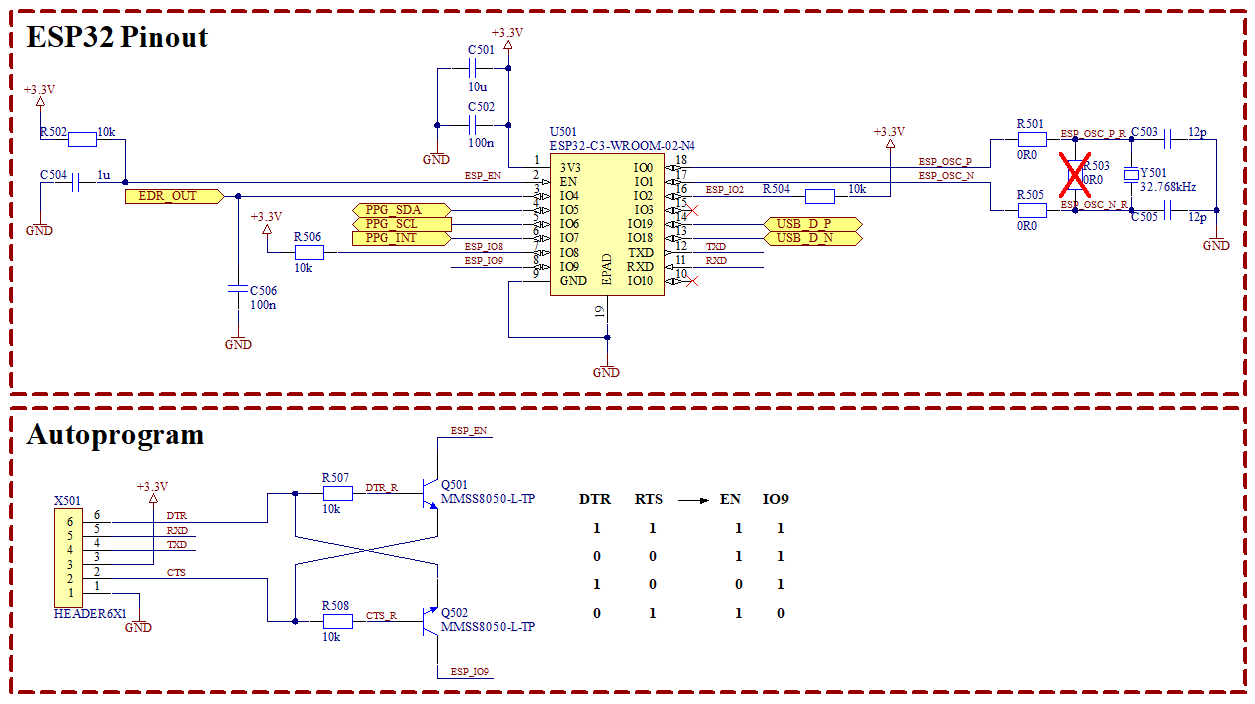
\includegraphics[width=1\textwidth]{Figures/BR_WIRELESS.png}
    \caption{Shema bežične komunikacije narukvice}
    \label{slk:BR_WIRELESS}
\end{sidewaysfigure}

\newpage
\section{Fotopletizmografski senzor}

Za mjerenje brzine otkucaja srca koristi se PPG senzor MAX30101 tvrtke Analog Devices (slika \ref{slk:MAX30101}). Ovaj snezor u sebi ima crvenu, zelenu i infracrvenu svjetleću diodu i fotosenzor, upravljačko sklopovlje za diode, te komunicira preko I\textsuperscript{2}C sučelja. Kao što je vidljivo na shemi na slici \ref{slk:PPG} ovaj senzor je veoma jednostavan za implementaciju uz svega par par priteznih otpornika i blokadnih kondenzatora. Jedina komplikacija dolazi u obliku napajanja od 5 V, koje je potrebno jer je pad napona na zelenoj svjetlećoj diodi specificiran na 3.3 V.
\begin{figure}[htb]
    \centering
    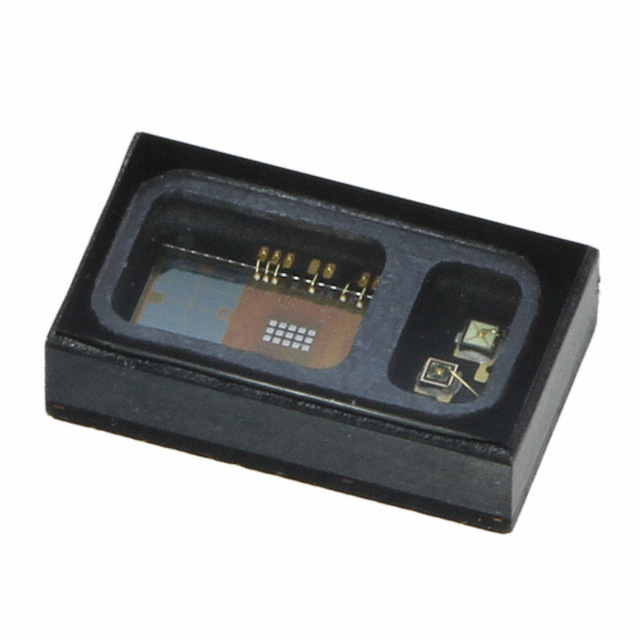
\includegraphics[width=6 cm]{Figures/MAX30101.JPG}
    \caption{MAX30101 PPG senzor}
    \label{slk:MAX30101}
\end{figure}
\begin{figure}[htb]
    \centering
    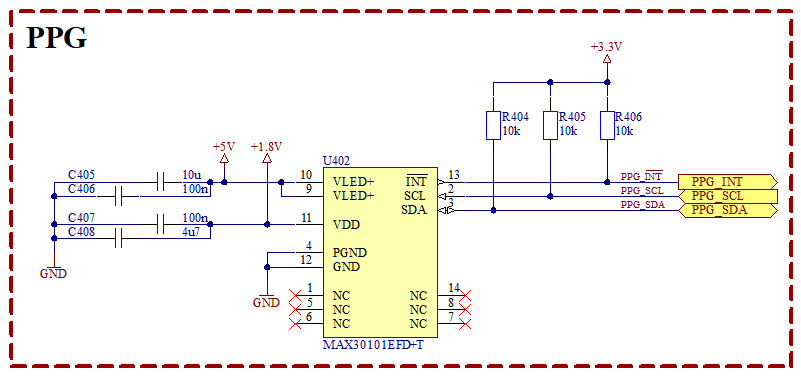
\includegraphics[width=\textwidth]{Figures/PPG.png}
    \caption{Shema PPG senzora}
    \label{slk:PPG}
\end{figure}

\section{Impedancija kože}